\documentclass[12pt]{article}
%%---------------------------------------------------------------------
% packages
% geometry
\usepackage{geometry}
% font
\usepackage{fontspec}
\defaultfontfeatures{Mapping=tex-text}  %%如果没有它,会有一些 tex 特殊字符无法正常使用,比如连字符。
\usepackage{xunicode,xltxtra}
\usepackage[BoldFont,SlantFont,CJKnumber,CJKchecksingle]{xeCJK}  % \CJKnumber{12345}: 一万二千三百四十五
\usepackage{CJKfntef}  %%实现对汉字加点、下划线等。
\usepackage{pifont}  % \ding{}
% math
\usepackage{amsmath,amsfonts,amssymb}
% color
\usepackage{color}
\usepackage{xcolor}
\definecolor{EYE}{RGB}{199,237,204}
\definecolor{FLY}{RGB}{128,0,128}
\definecolor{ZHY}{RGB}{139,0,255}
% graphics
\usepackage[americaninductors,europeanresistors]{circuitikz}
\usepackage{tikz}
\usetikzlibrary{positioning,arrows,shadows,shapes,calc,mindmap,trees,backgrounds}  % placements=positioning
\usepackage{graphicx}  % \includegraphics[]{}
\usepackage{subfigure}  %%图形或表格并排排列
% table
\usepackage{colortbl,dcolumn}  %% 彩色表格
\usepackage{multirow}
\usepackage{multicol}
\usepackage{booktabs}
% code
\usepackage{fancyvrb}
\usepackage{listings}
% title
\usepackage{titlesec}
% head/foot
\usepackage{fancyhdr}
% ref
\usepackage{hyperref}
% pagecolor
\usepackage[pagecolor={EYE}]{pagecolor}
% tightly-packed lists
\usepackage{mdwlist}

\usepackage{styles/iplouccfg}
\usepackage{styles/zhfontcfg}
\usepackage{styles/iplouclistings}

%%---------------------------------------------------------------------
% settings
% geometry
\geometry{left=2cm,right=1cm,top=2cm,bottom=2cm}  %设置 上、左、下、右 页边距
\linespread{1.5} %行间距
% font
\setCJKmainfont{Adobe Kaiti Std}
%\setmainfont[BoldFont=Adobe Garamond Pro Bold]{Apple Garamond}  % 英文字体
%\setmainfont[BoldFont=Adobe Garamond Pro Bold,SmallCapsFont=Apple Garamond,SmallCapsFeatures={Scale=0.7}]{Apple Garamond}  %%苹果字体没有SmallCaps
\setCJKmonofont{Adobe Fangsong Std}
% graphics
\graphicspath{{figures/}}
\tikzset{
    % Define standard arrow tip
    >=stealth',
    % Define style for boxes
    punkt/.style={
           rectangle,
           rounded corners,
           draw=black, very thick,
           text width=6.5em,
           minimum height=2em,
           text centered},
    % Define arrow style
    pil/.style={
           ->,
           thick,
           shorten <=2pt,
           shorten >=2pt,},
    % Define style for FlyZhyBall
    FlyZhyBall/.style={
      circle,
      minimum size=6mm,
      inner sep=0.5pt,
      ball color=red!50!blue,
      text=white,},
    % Define style for FlyZhyRectangle
    FlyZhyRectangle/.style={
      rectangle,
      rounded corners,
      minimum size=6mm,
      ball color=red!50!blue,
      text=white,},
    % Define style for zhyfly
    zhyfly/.style={
      rectangle,
      rounded corners,
      minimum size=6mm,
      ball color=red!25!blue,
      text=white,},
    % Define style for new rectangle
    nrectangle/.style={
      rectangle,
      draw=#1!50,
      fill=#1!20,
      minimum size=5mm,
      inner sep=0.1pt,}
}
\ctikzset{
  bipoles/length=.8cm
}
% code
\lstnewenvironment{VHDLcode}[1][]{%
  \lstset{
    basicstyle=\footnotesize\ttfamily\color{black},%
    columns=flexible,%
    framexleftmargin=.7mm,frame=shadowbox,%
    rulesepcolor=\color{blue},%
%    frame=single,%
    backgroundcolor=\color{yellow!20},%
    xleftmargin=1.2\fboxsep,%
    xrightmargin=.7\fboxsep,%
    numbers=left,numberstyle=\tiny\color{blue},%
    numberblanklines=false,numbersep=7pt,%
    language=VHDL%
    }\lstset{#1}}{}
\lstnewenvironment{VHDLmiddle}[1][]{%
  \lstset{
    basicstyle=\scriptsize\ttfamily\color{black},%
    columns=flexible,%
    framexleftmargin=.7mm,frame=shadowbox,%
    rulesepcolor=\color{blue},%
%    frame=single,%
    backgroundcolor=\color{yellow!20},%
    xleftmargin=1.2\fboxsep,%
    xrightmargin=.7\fboxsep,%
    numbers=left,numberstyle=\tiny\color{blue},%
    numberblanklines=false,numbersep=7pt,%
    language=VHDL%
    }\lstset{#1}}{}
\lstnewenvironment{VHDLsmall}[1][]{%
  \lstset{
    basicstyle=\tiny\ttfamily\color{black},%
    columns=flexible,%
    framexleftmargin=.7mm,frame=shadowbox,%
    rulesepcolor=\color{blue},%
%    frame=single,%
    backgroundcolor=\color{yellow!20},%
    xleftmargin=1.2\fboxsep,%
    xrightmargin=.7\fboxsep,%
    numbers=left,numberstyle=\tiny\color{blue},%
    numberblanklines=false,numbersep=7pt,%
    language=VHDL%
    }\lstset{#1}}{}
% pdf
\hypersetup{%pdfpagemode=FullScreen,%
            pdfauthor={Haiyong Zheng},%
            pdftitle={Title},%
            CJKbookmarks=true,%
            bookmarksnumbered=true,%
            bookmarksopen=false,%
            plainpages=false,%
            colorlinks=true,%
            citecolor=green,%
            filecolor=magenta,%
            linkcolor=cyan,%red(default)
            urlcolor=cyan}
% section
%http://tex.stackexchange.com/questions/34288/how-to-place-a-shaded-box-around-a-section-label-and-name
\newcommand\titlebar{%
\tikz[baseline,trim left=3.1cm,trim right=3cm] {
    \fill [cyan!25] (2.5cm,-1ex) rectangle (\textwidth+3.1cm,2.5ex);
    \node [
        fill=cyan!60!white,
        anchor= base east,
        rounded rectangle,
        minimum height=3.5ex] at (3cm,0) {
        \textbf{\thesection.}
    };
}%
}
\titleformat{\section}{\Large\bf\color{blue}}{\titlebar}{0.1cm}{}
% head/foot
\setlength{\headheight}{15pt}
\pagestyle{fancy}
\fancyhf{}

\chead{\color{black!50!green}Assignment \#3}

%\lfoot{\color{blue!50!green}Dai Jialun}
\cfoot{\color{blue!50!green}\href{http://vision.ouc.edu.cn/~zhenghaiyong}{CVBIOUC}}
\rfoot{\color{blue!50!green}$\cdot$\ \thepage\ $\cdot$}
\renewcommand{\headrulewidth}{0.4pt}
\renewcommand{\footrulewidth}{0.4pt}

%%---------------------------------------------------------------------
\begin{document}
%%---------------------------------------------------------------------
%%---------------------------------------------------------------------
% \titlepage
\title{\vspace{-2em} 浮游动物识别分类——深度学习\\
\normalsize{}}
\author{Dai Jialun \hspace{0.25in} Wu Bin}
\date{\vspace{-0.7em} \today \vspace{-0.7em}}
%%---------------------------------------------------------------------
\maketitle\thispagestyle{fancy}
%%---------------------------------------------------------------------
\maketitle
%\tableofcontents 
\section{Caffe }
Caffe(Convolutional Architecture for Fast Feature Embedding)是纯粹的C++/CUDA架构,支持命令行、Python和MATLAB接口,且在CPU和GPU直接无缝切换。
\subsection{Caffe优点:}
\begin{itemize}
\item 上手快:模型与相应优化都是以文本形式而非代码形式给出。
\item 速度快:能够运行较好的模型与海量的数据。
\item 模块化:方便扩展到新的任务和设置上。
\item 开放性:公开的代码和参考模型用于再现。
\item 社区好:可以通过BSD-2参与开发与讨论。
\end{itemize}




\subsection{代码层次}
\begin{description}
\item[\textbf{Blob}] 基础的数据结构,{\color{blue} 保存学习到的参数}以及{\color{blue} 网络传输过程中产生数据的类}。\\
	主要是对protocol buffer所定义的数据结构的继承,Caffe也因此可以在尽可能小的内存占用下获得很高的效率。在更高一级的Layer中Blob用下面的形式表示学习到的参数:
	\begin{itemize}
	\item vector<sharedptr<Blob<Dtype> > > blob
	\item vector<Blob<Dtype>*> \& bottom
	\item vector<Blob<Dtype>*> *top
	\end{itemize}
\item[\textbf{Layer}] 网络的基本单元,由此派生出了各种层类。修改这部分的人主要是{\color{blue} 研究特征表达}方向的。\\
	用某种Layer来表示卷积操作,非线性变换,Pooling,权值连接等操作。具体分为5大类Layer:
	\begin{itemize}
	\item \textbf{NeuronLayer} \hspace{0.1in} 定义于neuron\_layers.hpp中,其派生类主要是元素级别的运算,运算均为同址计算。
	\item \textbf{LossLayer} \hspace{0.1in} 定义于loss\_layers.hpp中,其派生类会产生loss,只有这些层能够产生loss。
	\item \textbf{数据层} \hspace{0.1in} 定义于data\_layer.hpp中,作为网络的最底层,主要实现数据格式的转换。
	\item \textbf{特征表达层} \hspace{0.1in} 定义于vision\_layers.hpp,实现特征表达功能,例如卷积操作,Pooling操作等。
	\item \textbf{网络连接层和激活函数(待定)} \hspace{0.1in} 定义于common\_layers.hpp,Caffe提供了单个层与多个层的连接,并在这个头文件中声明。这里还包括了常用的全连接层InnerProductLayer类。
	\end{itemize}
	在Layer内部,数据主要有两种传递方式,\textbf{正向传导(Forward)}和\textbf{反向传导(Backward)}。Caffe中所有的Layer都要用这两种方法传递数据。
\item[\textbf{Net}] 网络的搭建,{\color{blue} 将Layer所派生出层类组合成网络}。\\
Net用容器的形式将多个Layer有序地放在一起,其自身实现的功能主要是对逐层Layer进行初始化,以及提供Update()的接口(更新网络参数),本身不能对参数进行有效地学习。
	\begin{itemize}
	\item vector<shared\_ptr<Layer<Dtype> > > layers \_
	\item vector<Blob<Dtype>*> \& Forward()
	\item void Net<Dtype>::Backward()
	\end{itemize}
\item[\textbf{Solver}] Net的求解,修改这部分人主要会是{\color{blue} 研究DL求解}方向的。\\
	这个类中包含一个Net的指针,主要是实现了训练模型参数所采用的优化算法,它所派生的类就可以对整个网络进行训练了。
	\begin{itemize}
	\item shared\_ptr<Net<Dtype> > net\_
	\item virtual void ComputeUpdateValue() = 0
	\end{itemize}
\end{description}

\section{CNN}
Deep Learning是全部深度学习算法的总称,CNN是深度学习算法在图像处理领域的一个应用。

\subsection{CNN优点:}
\begin{itemize}
\item 权值共享网络结构,降低网络模型的复杂度,减少了权值的数量。
\item 图像直接作为网络的输入,避免复杂的特征提取和数据重建。
\item 对平移、比例缩放、倾斜或者其他形式的变形具有高度不变性。
\end{itemize}

\subsection{CNN组成:}
\begin{itemize}
\item 局部感知
\item 参数共享
\item 多卷积核
\item Down-pooling
\item 多层卷积
\end{itemize}


\subsection{CNN网络配置文件:}
\begin{itemize}
\item Imagenet\_solver.prototxt (包含全局参数的配置文件)
\item Imagenet.prototxt (包含训练网络的配置文件)
\item Imagenet\_val.prototxt (包含测试网络的配置文件)
\end{itemize}



\section{AlexNet}
\subsection{网络结构}
AlexNet网络结构是CNN类型的DeepLearning网络模型在图像分类上的应用,如图Figure~\ref{fig:framework}。

\begin{figure}[!ht]
\centering
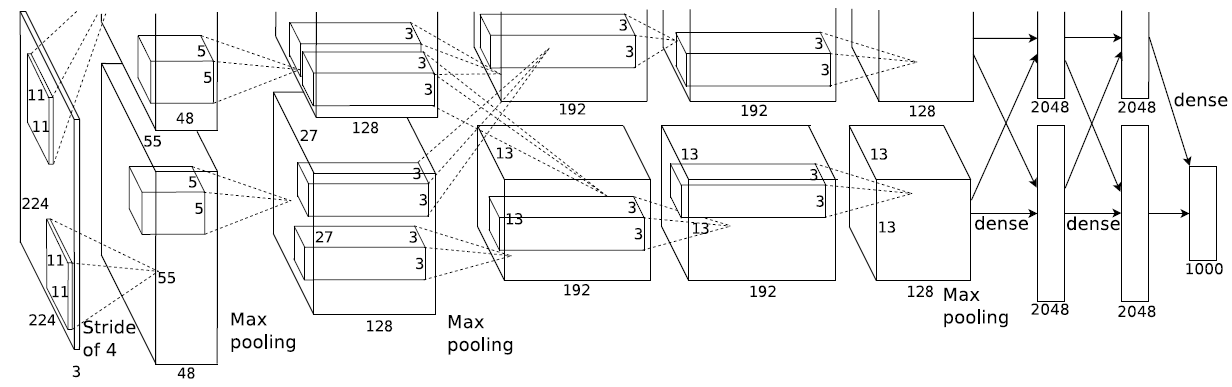
\includegraphics[width=0.8\textwidth]{AlexNet}
\caption{AlexNet}
\label{fig:framework}
\end{figure}

\begin{itemize}
\item 输入224$\times$224的图片,3通道
\item 第一层卷积 + pooling:11$\times$11的卷积核96个,步长为4,每个GPU各有48个。max-pooling的核为2$\times$2。如图Figure~\ref{fig:conv1}。
	\begin{figure}[!ht]
	\centering
	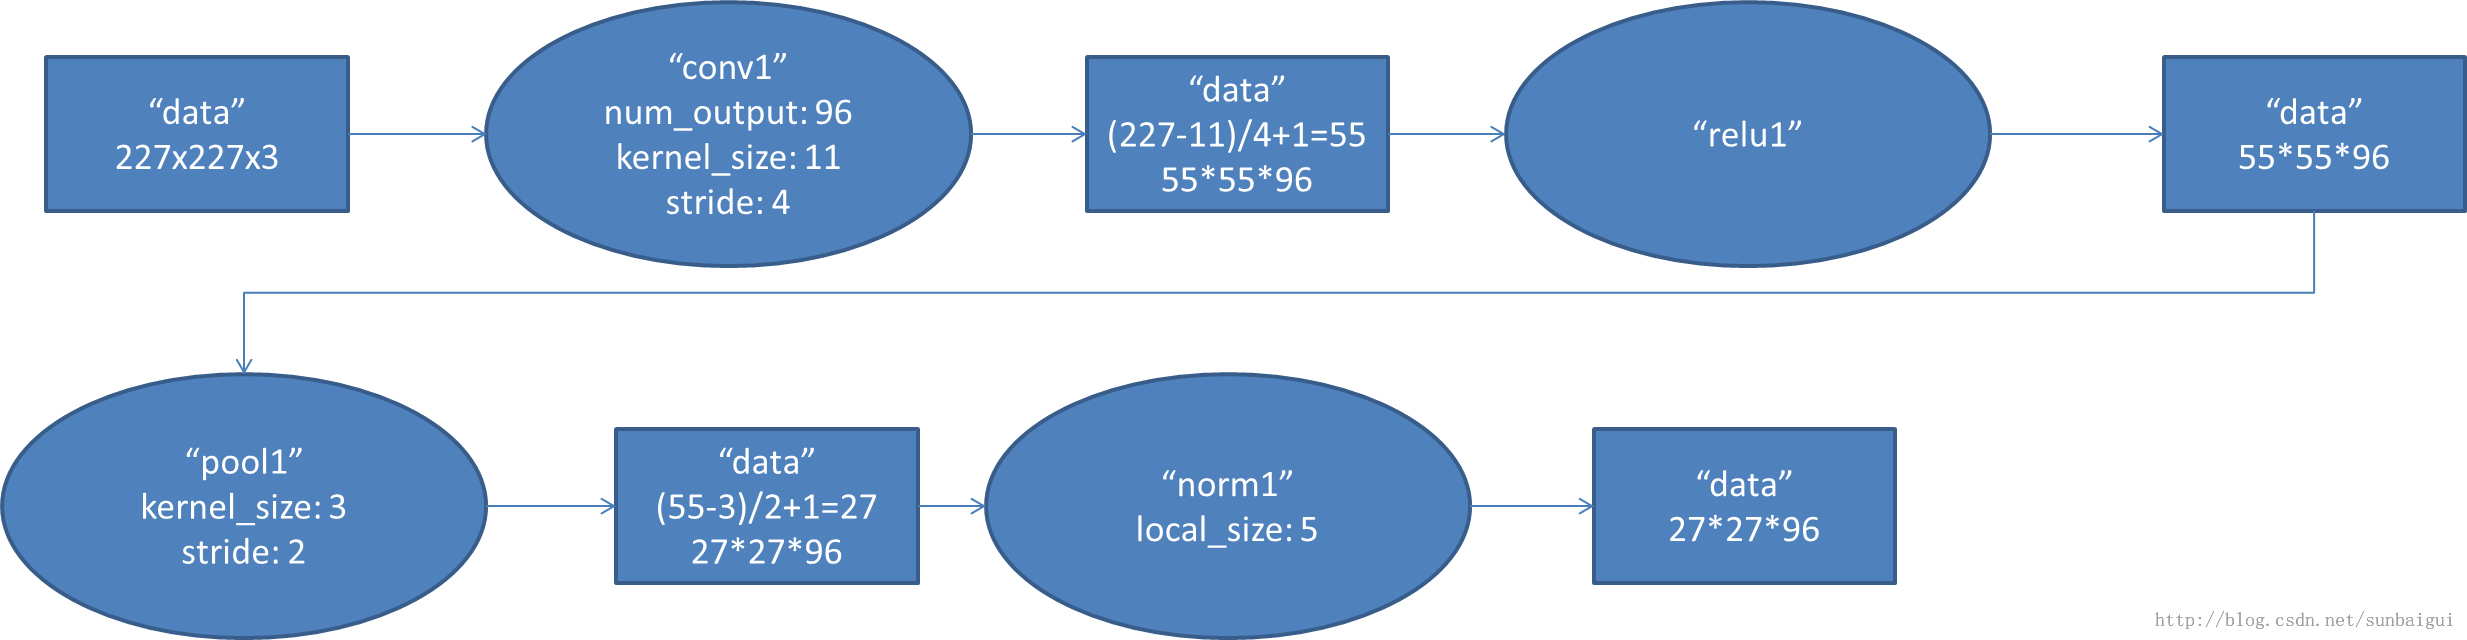
\includegraphics[width=0.7\textwidth]{conv1_1}
	\caption{Conv1}
	\label{fig:conv1}
	\end{figure}
\end{itemize}

\begin{itemize}
\item 第二层卷积 + pooling:5$\times$5的卷积核256个,每个GPU各有128个。max-pooling的核为2$\times$2。如图Figure~\ref{fig:conv2}。
	\begin{figure}[!ht]
	\centering
	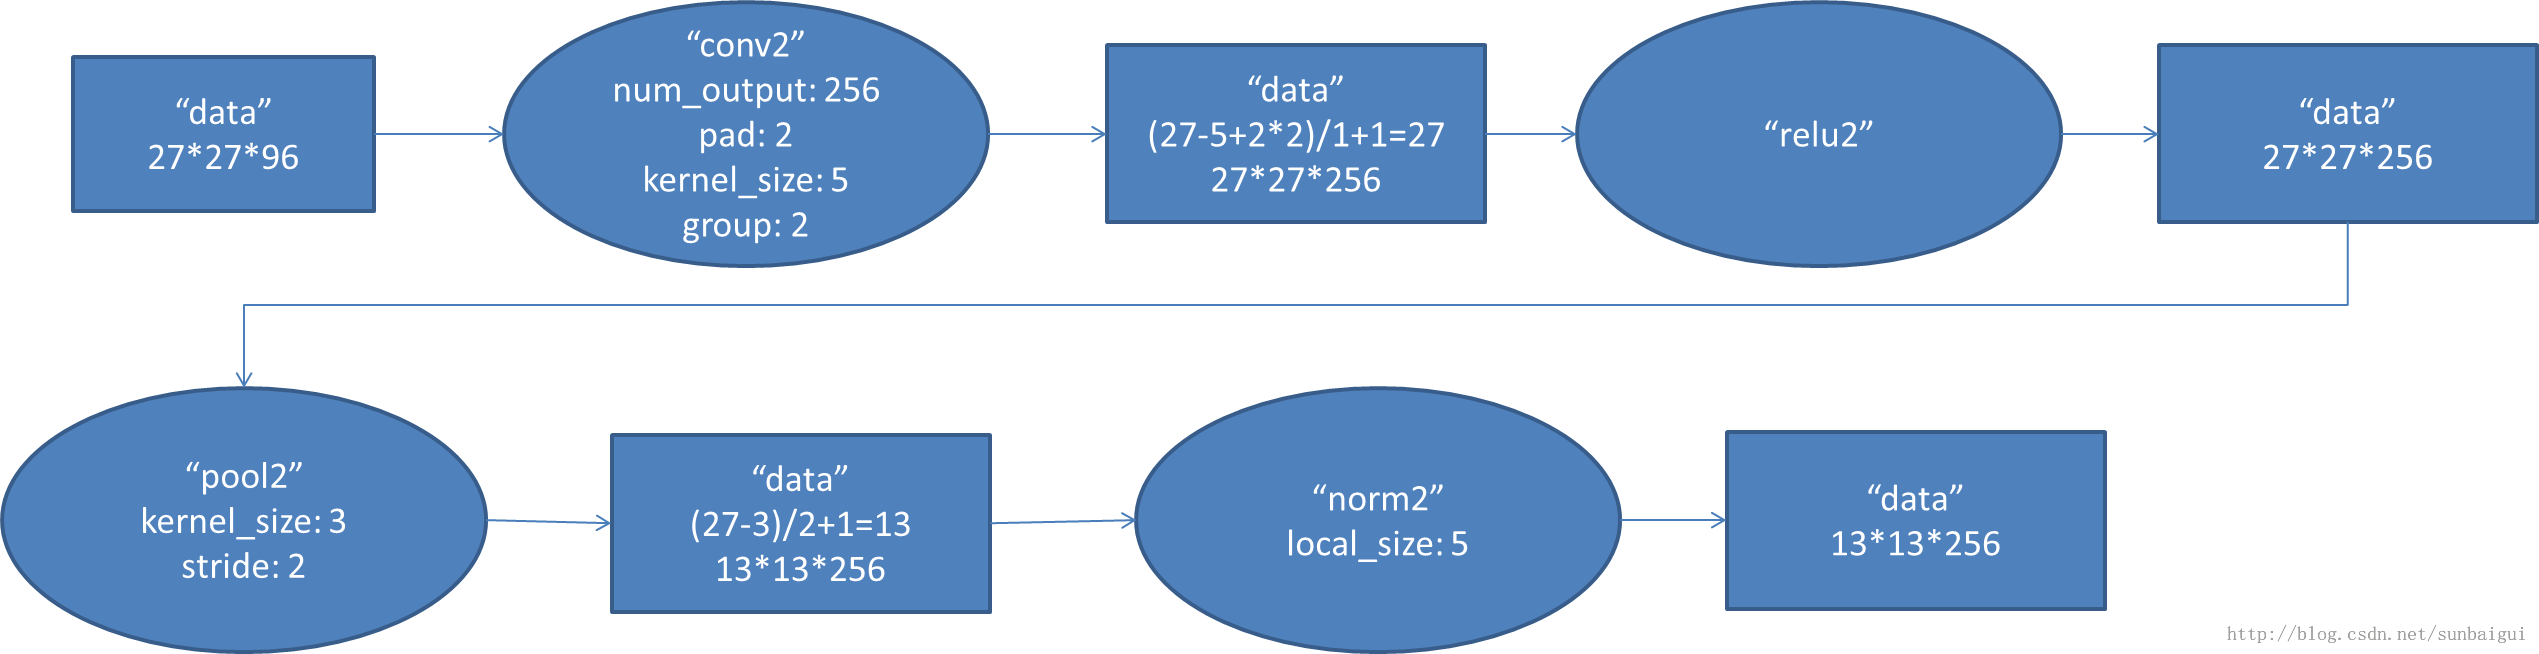
\includegraphics[width=0.7\textwidth]{conv2_2}
	\caption{Conv2}
	\label{fig:conv2}
	\end{figure}
\end{itemize}

\begin{itemize}
\item 第三层卷积:与上一层是全连接。3$\times$3的卷积核384个,每个GPU各有192个。如图Figure~\ref{fig:conv3}。
	\begin{figure}[!ht]
	\centering
	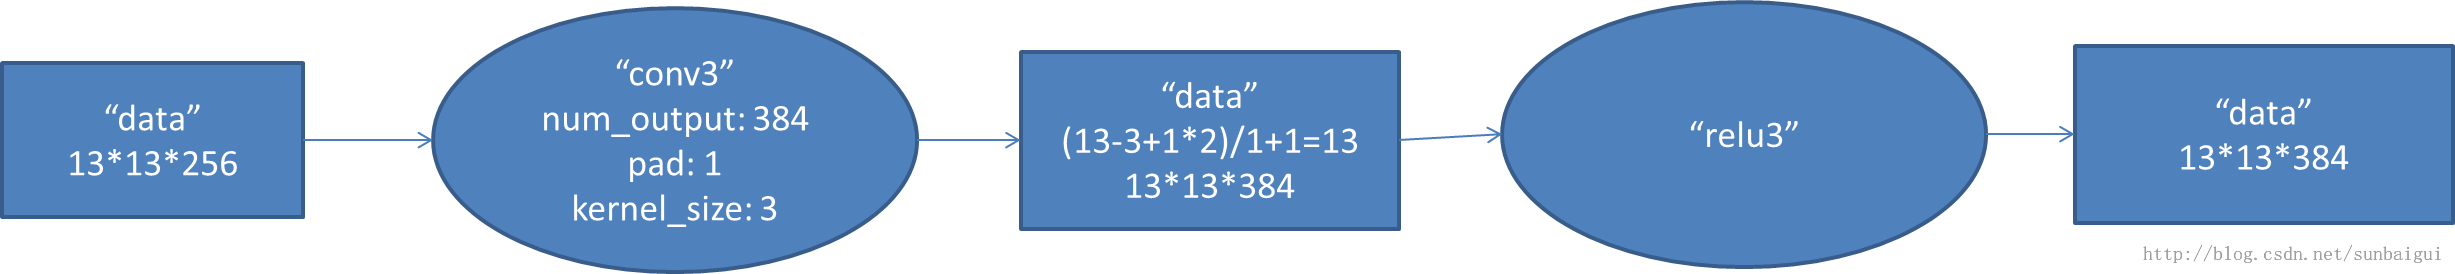
\includegraphics[width=0.7\textwidth]{conv3}
	\caption{Conv3}
	\label{fig:conv3}
	\end{figure}
\item 第四层卷积:3$\times$3的卷积核384个,每个GPU各有192个。如图Figure~\ref{fig:conv4}。
	\begin{figure}[!ht]
	\centering
	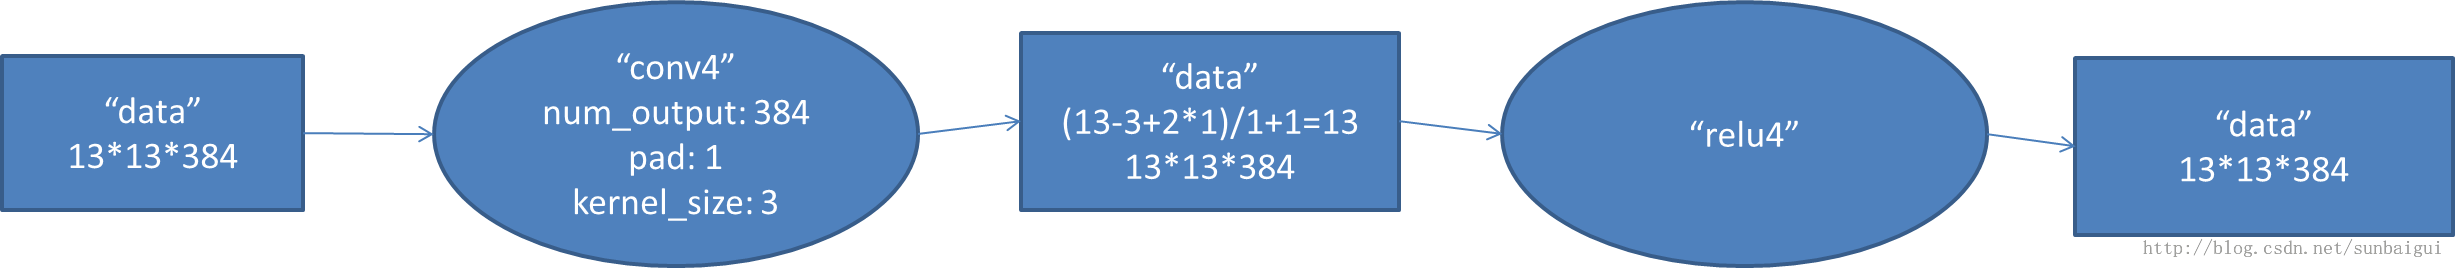
\includegraphics[width=0.7\textwidth]{conv4}
	\caption{Conv4}
	\label{fig:conv4}
	\end{figure}
\item 第五层卷积 + pooling:3$\times$3的卷积核256个,每个GPU各有128个。max-pooling:2 $\times$2的核。如图Figure~\ref{fig:conv5}。
	\begin{figure}[!ht]
	\centering
	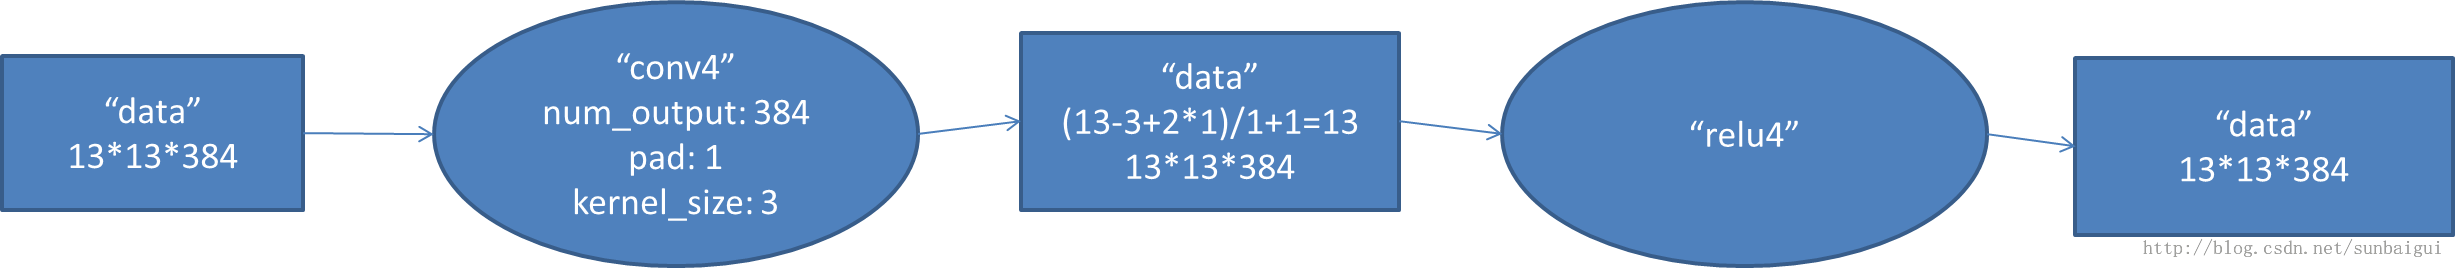
\includegraphics[width=0.7\textwidth]{conv4}
	\caption{Conv5}
	\label{fig:conv5}
	\end{figure}
\end{itemize}

\begin{itemize}
\item 第六层全连接:4096维,将第五层的输出连接成为一个一维向量,作为该层的输入。如图Figure~\ref{fig:fc6}。
	\begin{figure}[!ht]
	\centering
	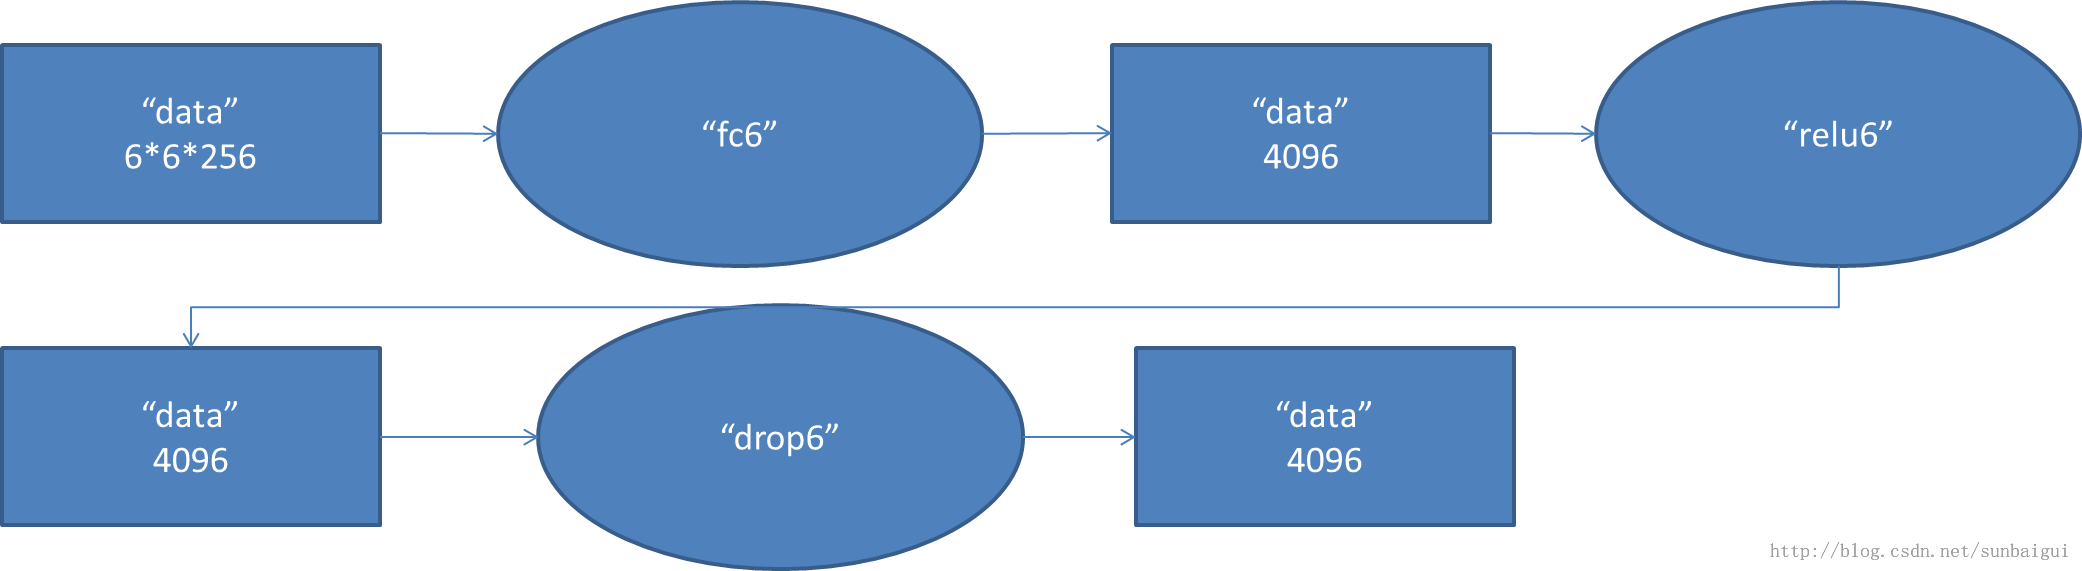
\includegraphics[width=0.7\textwidth]{fc1}
	\caption{Fc6}
	\label{fig:fc6}
	\end{figure}
\item 第七层全连接:4096维,将第六层的输出连接成为一个一维向量。如图Figure~\ref{fig:fc7}。
	\begin{figure}[!ht]
	\centering
	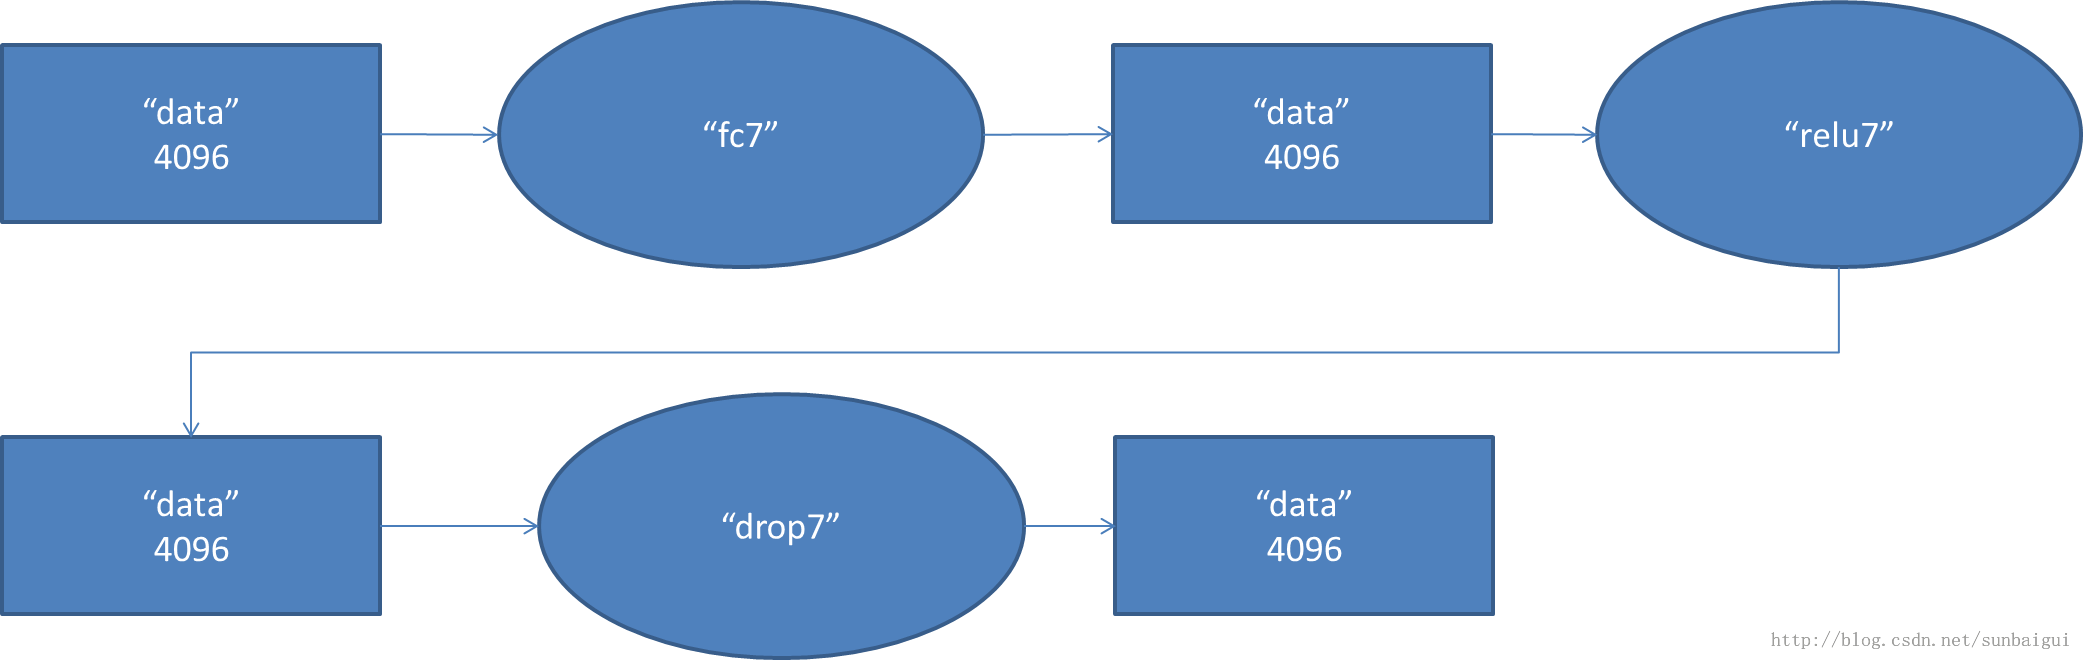
\includegraphics[width=0.7\textwidth]{fc2}
	\caption{Fc7}
	\label{fig:fc7}
	\end{figure}
\item Softmax层:输出为1000,输出的每一维都是图片属于该类别的概率。如图Figure~\ref{fig:fc8}。
	\begin{figure}[!ht]
	\centering
	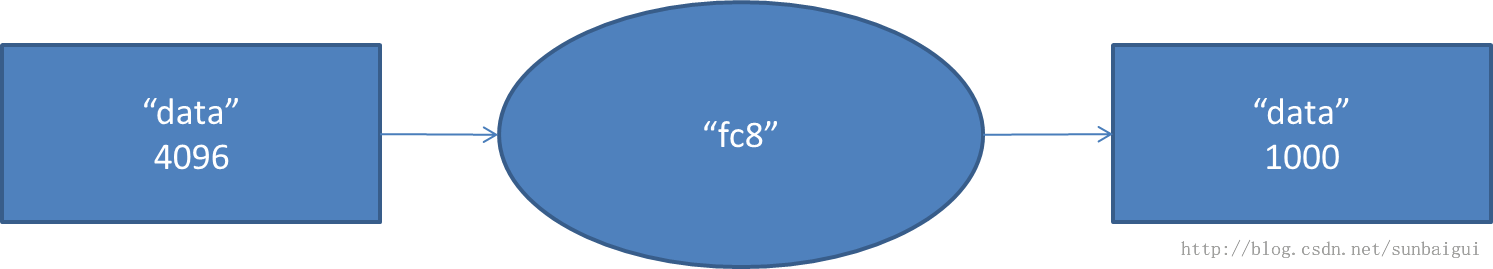
\includegraphics[width=0.7\textwidth]{fc3}
	\caption{Fc8}
	\label{fig:fc8}
	\end{figure}
\end{itemize}

\subsection{在数据与模型上的技巧}
\begin{itemize}
\item 数据
	\begin{itemize}
	\item 增大训练样本
	\item 用PCA增强训练数据
	\end{itemize}
\item 模型结构
	\begin{itemize}
	\item Local Response Normalization
	\item Dropout策略
	\end{itemize}
\item 优化算法的参数
	\begin{itemize}
	\item SGD(随机梯度下降法)
	\end{itemize}
\end{itemize}
%%---------------------------------------------------------------------
\end{document}
